\chapter{Design}
-objectives
-use cases (actors)
-architecture of backend
-design patterns
-gui (with screenshots)
\par For the design, a clear set of objectives, use cases and architecture have been developed to aid the implementation.
\section{Objectives}
\par The Objectives of the system are for it to be visible, efficient, and effective.
\par \textbf{Visible} -  It should be visible to the user what  functions are available. This includes being able to distinguish actions from informative text. Thereby, providing an application that can be picked up and used with minimal to no training and benefiting the growth of users of the system. This can be achieved by providing a simple and intuitive User Interface (UI), where buttons are highlighted, and actions are not cluttered, instead only necessary actions are provided. 

\par \textbf{Efficient} - The time spent to perform tasks should be reasonable in the context of its input. This can be further expressed in the mathematical notation of Big-Oh. If an algorithm takes an input of size $n$, and roughly performs $n$ operations to produce a result, then the algorithm is said to have a runtime of Big-Oh of $n$ (visually shown as $O(n)$). This allows the efficiency to be compared between algorithms, as the focus is on how well they scale with larger inputs. The objective is to not have an algorithm that processes the files with an exponential time complexity. With an exponential time complexity, a small $n$ would lead to a large running time, therefore a larger $n$ would result in an infeasible running time. Threads can be used to aid this task. A Thread is a lightweight processor computation unit. Using more than one-thread allows for tasks to be carried out in parallel. Therefore, if the input is $n$ documents, and there are $n$ threads, then the running time of the system would be the greatest running time of all the documents being carried out. Since all documents are being processed in parallel, completely independently of each other, then the time of the document that takes the longest time to process would result in the time it takes to process the entire set of documents.

\par \textbf{Effective} - The system should meeet its purpose. Which is to require as input documents and process them to produce a timeline. The system should allow the user to perform these tasks through menu options, buttons, and, in addition, produce appropriate responses. When an error occurs the system should not attempt to process the documents idefinetely, and instead produce a timeline with the available events. Effectiveness also involves how correct are the timelines poduced by the system. Whether they provide the user the correct information, and if the events are being identified in the documents. 

\section{Use Cases}
\par A use case is a task an actor in the system performs. An actor is any type of user of the system. In this case, the user can be a law professional that uses the system to have a general understanding of a set of documents. Therefore, it can be assumed that the user does not necessarily have experience with NLP. It should be transparent to the user how the documents are being parsed, and only if they are interested would they require to look at the available source-code. The technical skill of the user does not need to be of an expert, as the tasks required are to provide documents, and view and interact with the produced timeline. In some cases, the user may produce their own graphical representation of a timeline and just use the produced JSON of the system. This would be the case if they have develoed their own system to interact with this system.
\par The use cases of the system are given by the requirements, and they are presented below. //use case stick figure diagram
\begin{enumerate}
  \item Load Documents
  \begin{enumerate}
    \item Primary Actor: User
    \item Goal: load set of given documents, where the document file types can be  .pdf, .docx, or .txt.
    \item Main Sequence:
	\begin{enumerate}
		\item User selects the "Load Documents" option.
		\item System prompts a File Selector.
		\item User selects set of documents and the base dates (or reference dates) to use with them.
		\item System responds with timeline of events.
	\end{enumerate}
  \end{enumerate}
  \item Swap from Timeline to Document
   \begin{enumerate}
	\item Primary Actor: User
	\item Goal: show the sentence, in context, that produced the given event.
	\item Main Sequence:
	\begin{enumerate}
		\item User selects event.
		\item System responds with dialog to "Edit Event" or "Go to Document".
		\item User selects "Go to Document" option.
		\item System opens new window with the text of the document where the event originates from, with the sentence that produced it highglighted.
	\end{enumerate}
    \end{enumerate}
   \item Edit Event
      \begin{enumerate}
	\item Primary Actor: User
	\item Goal: modify the data of an event.
	\item Main Sequence:
	\begin{enumerate}
		\item User selects event.
		\item System responds with dialog to "Edit Event" or "Go to Document".
		\item User selects "Edit Event" option.
		\item System responds with dialog with the data of the event set in fields.
		\item User edits the data as needed.
		\item System validates the entered data, and saves.
	\end{enumerate}
     \end{enumerate}
   \item Save Timeline
    \begin{enumerate}
	\item Primary Actor: User
	\item Goal: save the produced timeline as a PDF or JSON.
	\item Main Sequence:
	\begin{enumerate}
		\item User selects "Save To..." option.
		\item System responds with option dialog to select the file format to save.
		\item User selects the needed file format.
		\item System responds with File Selector.
		\item User selects the location to save the timeline.
		\item System generates the required data to save the timeline in the desired format and attempts to save it in the system.
	\end{enumerate}
    \end{enumerate}
\end{enumerate}
//note load documents use case includes adding to an existing timeline, user is the person using the system, edit event incl delete, checks for invalid data, file not available
\par The main sequence are the steps of the interaction in the use case to reach the goal. An error can occur during the interaction, it should be the systems responsibility to deal with the error appropriately, and not end the execution of the program. The primary actor, is the agent or entity that initiates the use case (cite or footnote).
\par Note that loading documents includes both when it is the first set of documents to be loaded, i.e. the timeline is empty, and when there is already a populated timeline. In the latter case, it would be beneficial to discard duplicated events. A duplicated event is one where it is produced from the same file, using the same reference date, and the data is equal. This is done to not clutter the timeline with events that are repeated, as the timeline should be efficient in the data it provides, i.e. describe the events in the document with as little as possible of additional data. It can occur that two documents produce the same event, these should not count as duplicated, as the event may have a different context depending on what file they originate from. Reference dates are included in the check of duplicate events as it may be the case that different events are produced for the same document when different reference points are used, and the user is interested in investigating this. 

\par When an event is being edited, the user should have the option to delete it, as it may be that the system produced an erroneous event or the event is not relevant to the user. Events may not be relevant to the user if the same event occurs in two separate documents. This can occur when the events described in the documents overlap. The duplicate check would not identify them as duplicates as they originate from different files. To ensure the date entered by the user is correct, it is validated. The validation checks are carried out before the changes are saved.An example of invalid data is when the date of an event is modified but instead of a new date being set, other text data is entered. In the case of the event occuring during a range of dates, i.e. it has a start date and end date, a validation check should be that the second date does not occur before the first. The checks should be carried out before the data is saved. in the case the validation fails, the changes should not be changed, instead the user should be prompted to correct their input.
\par During the saving use case, the desired location can be unvailable. This can be either because the Operating System does not allow the alpplication to write to that directory, or because a file that is in use is being overwritten (i.e. a lock has been placed on it). Therefore, the user should be prompted to save in another location.

\section{Architecture}
\par The architecture of a system, is the structure of the components in the system\footnote{\url{https://msdn.microsoft.com/en-gb/library/ee658098.aspx}}. The focus is on the back-end, or logic, of the system as opposed to the graphical, or front-end. A good software architecture is one where the components of the system are encapsulated with other related components. For this project, the software architecture has been produced using Unified-Modelling Language (UML). In UML, components or classes are represented by a rectangle, with their available functions listed. The architecture of the whole system is presented in the figure below (Figure \ref{fig:fullArch}). Each package will be looked at individually.
\begin{figure}[H]
\caption{Full UML Architecture of Automated Timeline Extraction system.}
\label{fig:fullArch}
\includegraphics[width=\linewidth]{fullarch.png}
\centering
\end{figure}
\subsection{Process Package}
\par The core of the system is the process package (see Figure \ref{fig:process}). The architecture used here is Business Delegate, where all the interaction to the package is through one component, ProcessFiles, which delegates the work to the other components in the package. A list of files is passed in, along with their data (such as the file name, its path, or the creation/reference date used). Each file is processed in parallel. The maximum number of parallel processing allowed is given by the settings of the system (in the settings package). This is the maximum number of threads that can be ran at any given point. However, in the implementation one more thread should be added to the count, as the graphical user interface always runs on a separate thread. The belief is that with a maximum setting of $n$ threads, then at any given point at most $n$ files are being processed. Whenever one file finishes processing, another begins to be processed. As mentioned before, if $n$ files are allowed to process at any given point, and the input size of documents is $n$, then the time it takes for the system to process all the documents is given by the greates maximum time to process one of the $n$ files. The pseudo-code for this is given below (see Algorithm \ref{alg:processFiles}), in the implementation semaphores can be used to aid this task. A semaphore is a data structure that limit how many threads run by requiring threads to acquire a lock before performing their parallel processing. The lock is released afterwards by the thread. If no locks are available, threads wait until a lock is available.
\begin{figure}[H]
\caption{UML of the Processing Package}
\label{fig:process}
\includegraphics[width=\linewidth]{process.png}
\centering
\end{figure}
\begin{algorithm}
\SetKwInOut{Input}{Input}
\SetKwInOut{Output}{Output}
\Input{A list of Files to Process}
\Output{A list of Results}
\ForEach{File in the input list}{
	wait until can run\; \tcc{if the maximum number of threads running in parallel has not been reached then stop waiting, else wait}
	process the file\;
	add the produced Result to the list of Results to return\;
}
return list of Results\;
\caption{Algorithm for processing a list of Files}
\label{alg:processFiles}
\end{algorithm}
\par For this system, an event is described as a Result that contains date information (represented by TimelineDate), a set of subjects (or key words), and the summary of the sentence that produced the event.
\par The TimelineDate component processes temporal expressions identified by the Engine, these are parsed and an exact date is produced which is then used to compare and sort the Results(events).
\par In this system, the StanfordCoreNLP suite \footnote{\url{http://stanfordnlp.github.io/CoreNLP/}} is used. It is a well-known and tested tool for NLP. Other tools exist, such as ApacheNLP, however Stanford's tool has a larger set of documentation and support, as well as being thread-safe and efficient. Thread-safe refers to the ability to share this tool between separate processes without having to worry about concurrency issues. 
\par When a file is processed, its text is extracted, which is then parsed through the Engine. The Engine is responsible for producing the Results for a file. It identifies sentences with dates, and for those extracts subjects such as people, locations, money, etc. As well as using the Hedge-Trimmer algorithm, discussed in the Background Chapter, to produce a summary.

\subsection{System Package}
//talk about system to be shared throughout the system (same data shared)
\par The system package holds the system and settings components (see Figure \ref{fig:system}). It is responsible for providing global settings, such as the maximum number of threads to be ran in parallel, the threshold value used in the summary algorithm, and graphical settings. The SystemState attribute is used to identify at which stage the system is in when it is processing files. This allows for the logic of the system to be decoupled from the graphical representation, as it can use the system state to determine which actions are available, when a loading bar needs to be shown, and when the timeline is ready to be displayed. The component is shared throughout the system, as it contains data required in different components (both logical and graphical components).
\begin{figure}[H]
\caption{UML of the System Package}
\label{fig:system}
\includegraphics[width=\linewidth]{system.png}
\centering
\end{figure}

\subsection{Ranges Package}
//trees of ranges with results, algorithm, example, running time
\par The ranges package was the last package developed(see Figure \ref{fig:ranges}). It focuses on placing Results into ranges (see the Algorithm \ref{alg:produceRanges}), hence the name. A Range is defined by a start and end date. A Result is placed within this Range if it has the exact same start and end date, if this is not the case then it is attempted to place the Result in one of the children of this Range. If this is not possible, then another Range root is checked. Since Ranges are similar to Trees (as they recursively include other Ranges), there may be a fores of Ranges in the system. The roots is a Range with the largest range of dates that encupsalets its child Ranges (and their Results). Thereby allowing to group related events together, and encapsulating them by their dates.  
\begin{figure}[H]
\caption{UML of the Ranges Package}
\label{fig:ranges}
\includegraphics[width=\linewidth]{ranges.png}
\centering
\end{figure}
\begin{algorithm}
\SetKwInOut{Input}{Input}
\SetKwInOut{Output}{Output}
\Input{A list of Results}
\Output{A list of Range roots, i.e. a forest of Ranges}
sort the list of Results by the number of days in between the start and end date in descending order\;
\ForEach{Result in the sorted list}{
	attempt to add it to one of the existing Range roots\;
	\If{failed to add to existing Range}{
		make a new Range using the data of the Result\;
		add the new Range to the list of Range roots\;
	}
}
return list of Range roots\;
\caption{Algorithm for placing Results in Ranges}
\label{alg:produceRanges}
\end{algorithm}
\par The algorithm proceeds as follows. The Results are sorted by the range, the number of days between their start and end date. A Result that only has one date, has a range of 0. The Results with the largest ranges are added first as it is more likely that they encapsulate other Results (does not apply the other way round). This leads to the production of a tree, shown below. The root is a Range with a start and end date that encapsulates all the dates of its child Ranges. It may be necessary to expand the dates of a Range if it is the case that the dates of a Result partially overlap a Range. An expanded Range has no results, but has two children: the newly made Range for the Result that was being added, and the Range that the Result was previously partially overlapping.

\par To demonstrate the algoritm an example will be presented with the two Results presented in the table \ref{fig:resultsTable} and the pre-existing tree in Figure \ref{fig:rangeTreePre}. First, the Results would be sorted by their range, such that the second result is the first to be added. This produces the tree in Figure \ref{fig:rangeTree1}. Then the next Result in the table is added, producing the tree in Figure \ref{fig:rangeTree2}. For the resulting tree, it was determined that the Result  being added overlapped an existing Range, threby a new Range was formed that would encapsulate the previous Range and the result being added. This is done by extending the start and end dates appropriately. To place the Result in the tree after the Range was expanded, a new Range was created to hold it, and the previous Range that was partially being overlapped is now a child of the expanded Range.
\par As can be seen from the tree produced, the largest start-end date pair encapsulates the smaller start-end date pair, this can be done recursively. This allows for a graphical representation where the events are encapsulated by their dates, providing an alternative view to the traditional top-down timeline.
\begin{figure}[h]
\begin{center}
\begin{tabular}{ |c|c|c| } 
 \hline
Result & Start Date & End Date \\
\hline
\hline
1 & 12-12-2016 & 18-12-2016 \\
2 & 13-12-2016 & 20-12-2016 \\
 \hline
\end{tabular}
\end{center}
\caption{Example Results Start and End Date}
\label{fig:resultsTable}
\end{figure}
\begin{figure}[h]
\resizebox{\linewidth}{!}{
\Tree
 [.{01-01-1980  $\shortrightarrow$ 31-12-2016}
	[.{01-01-2008  $\shortrightarrow$ 31-05-2016} {01-01-2015} ]
	[{01-11-2016} ] 
]
}
\caption{Pre-existing Range Tree}
\label{fig:rangeTreePre}
\end{figure}
\begin{figure}[h]
\resizebox{\linewidth}{!}{
\Tree
 [.{01-01-1980 $\shortrightarrow$ 31-12-2016}
	[.{01-01-2008  $\shortrightarrow$ 31-05-2016} {01-01-2015} ]
	[{13-12-2016  $\shortrightarrow$ 20-12-2016} ]
	[{01-11-2016} ] 
]
}
\caption{Resulting Range Tree after adding the Result: 13-12-2016  $\shortrightarrow$ 20-12-2016}
\label{fig:rangeTree1}
\end{figure}
\begin{figure}
\resizebox{\linewidth}{!}{
\Tree
 [.{01-01-1980 $\shortrightarrow$ 31-12-2016}
	[.{01-01-2008  $\shortrightarrow$ 31-05-2016} {01-01-2015} ]
	[.{12-12-2016  $\shortrightarrow$ 20-12-2016} 
		[{12-12-2016  $\shortrightarrow$ 18-12-2016} ]
		[{13-12-2016  $\shortrightarrow$ 20-12-2016} ]
	]
	[{01-11-2016} ] 
]
}
\caption{Resulting Range Tree after adding the Result: 12-12-2016 $\shortrightarrow$ 18-12-2016}
\label{fig:rangeTree2}
\end{figure}

\subsection{Helpers Package}
\par The helper package  utility components required throughout the system (see Figure \ref{fig:helpers}). For example, it provides sorting functions (sorting by the start date or by the range of days in between the start and end date) and saving the timeline in PDF or JSON format. It is a refactored package of reused logic in the system. Refactoring is done to remove repeated components and operations. Thereby having them in one place only instead of being duplicated around the system. The main advantage is that when a change needs to be made, it is made in one place, but if the operations are duplicated throughout the system then that change needs to be carried out at each duplicated occurrence.
\begin{figure}[H]
\caption{UML of the Helpers Package}
\label{fig:helpers}
\includegraphics[scale=0.75]{helpers.png}
\centering
\end{figure}

\section{Design Patterns}
\par Design Patters are general solutions to common problems in software development\footnote{\url{https://sourcemaking.com/design_patterns}}. The solutions usually include a system architecture to follow. For this project, the main design patterns are Singleton and Observer.
\par \textbf{Singleton} - This design pattern ensures that only a certain number of instances of a component are available\footnote{\url{http://www.journaldev.com/1377/java-singleton-design-pattern-best-practices-examples}}. In most cases the number of components is restricted to one. The advantage of this pattern is to provide a universal access for global data throughout the system. For example, in the System component the NLP processing tool is held, along with the system state. These are both used throughout the system, hence it would reasonable to use a Singleton pattern to ensure their availability, and not reload them into memory each time.
\par \textbf{Observer} - This design pattern allows an observee to notify a list of its observers. The observee can be a model, and the the observers its view. This is used to separate the logic of the system from its user interface. It allows for the back-end of the system to be developed completely independently from the front-end. In this system, the front-end will be notified by the back-end. This is then strengthened further through the system states available. As the back-end begins processing documents, its state changes. The front-end should then change appropriately in such case, by retrieving the relevant data and showing the relevant for that state. If the system were to be developed further, with other graphical interfaces used or added to the pre-existing UI, then these could be added effortlessly as the logic of the system is independent of its view.
\par \textbf{Model-View Controller} - It is mentioned as a main design pattern of the system, because it is similar to the Observer design pattern, in that it separates the view from the data (which is a model) through a controller. The controller manipulates the data, and applies the appropriate changes in the view. It separates the logic of the system with its view, like an Observer pattern. This design pattern is enforced by many Graphical User Interface (GUI) frameworks, incluiding the one used in this project (JavaFX\footnote{\url{http://docs.oracle.com/javase/8/javase-clienttechnologies.htm}}). 
\par Other design patterns are available, however these are the most relevant ones for this project. While the solution to ensure safe multi-threading is not a design pattern, it is worth mentioning as it allows for safe independent processing of documents through the use of semaphores (mentioned previously). 
//singleton, model-view-controller, describe, explain why, and what other options were available
\section{UI}
\par The system is intended to be used by law professionals. However, it can be used by anyone that requires its services of producing timelines, as it will be open-source.  These considerations are taken into account during the development of the User-Interface. For example, as the main data representation of the system is the timeline of events, it is clear that it should occupy the majority of the screen. Options that are not relevant to the current state of the system should not be available, while options that are most likely to be used should be highlighted. The aim is to build a UI that is visible and easy to use for the user.
\par Actions that are made unavailable ensure that the user is not overloaded with buttons and menu options that do not make sense within the current state of processing the system is in. For example, when the system is initially launched, no timeline can be presented as no documents are available to be processed. Instead the user is invited to load documents, as can be seen by the Wirefram Figure \ref{fig:startup}. Wireframes are colourless screenshots of what the UI of a system should aim to look like, it is used by the front-end designers.
\begin{figure}[h]
\caption{Wireframe of System at Startup}
\label{fig:startup}
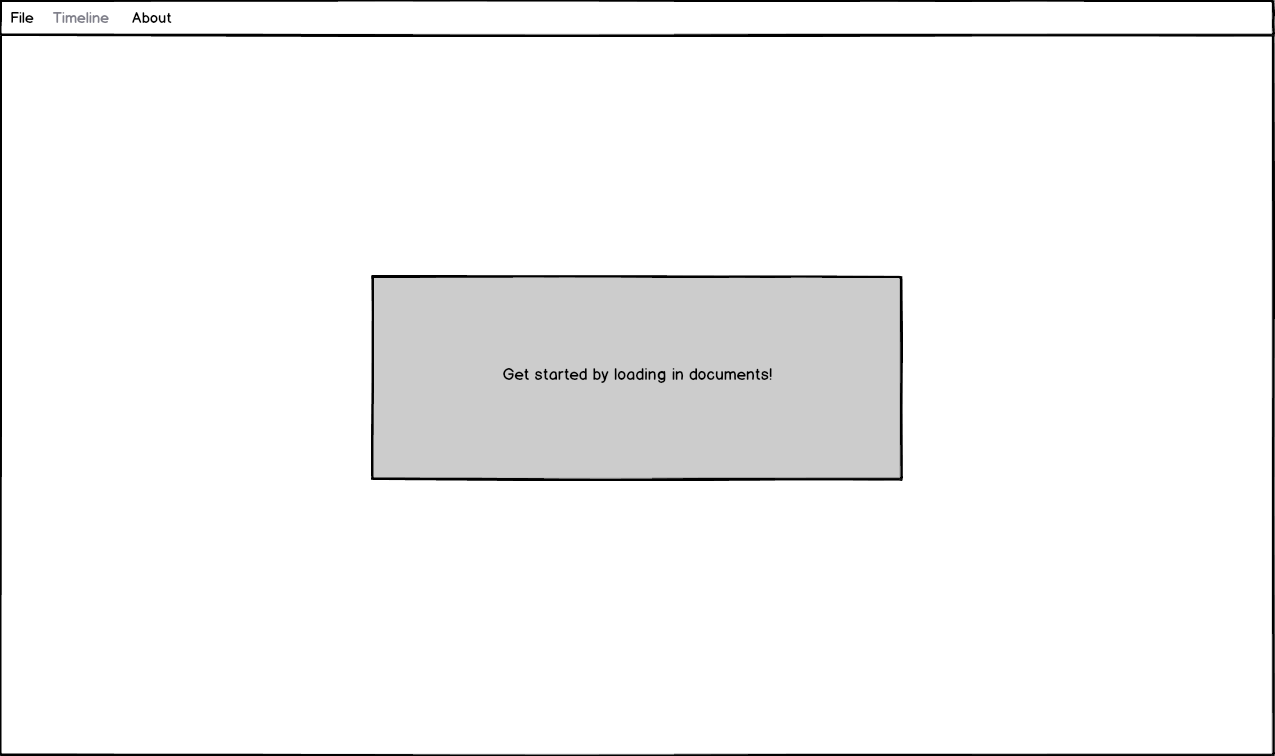
\includegraphics[width=\linewidth]{startup.png}
\centering
\end{figure}
\par From the start up screen, the user can load documents and the reference points used for the documents through a dialog displayed after the files have been selected. As this is being done, the system can load any resources it requires (such as models) before the files are to be processed. After the documents have been processed, the timeline is displayed (see Figure\ref{fig:timeline}).
\begin{figure}[h]
\caption{Timeline of System}
\label{fig:timeline}
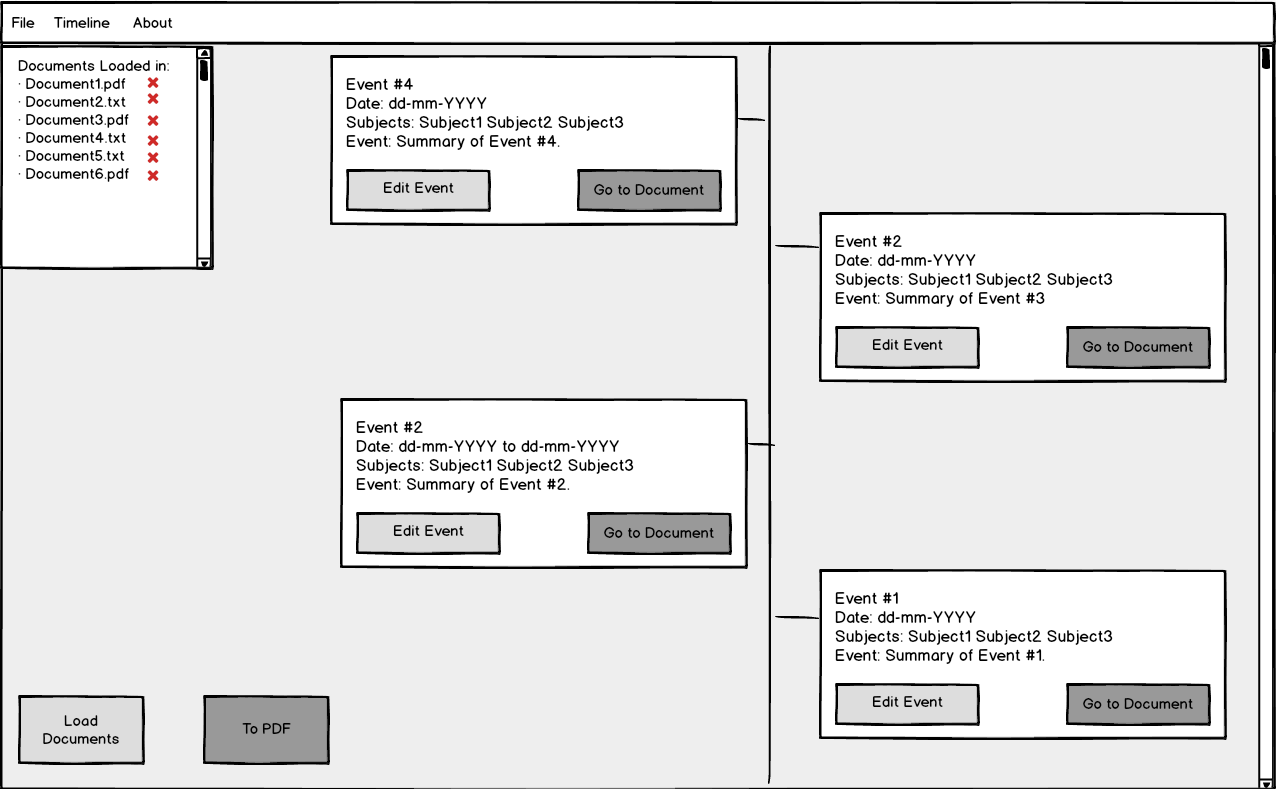
\includegraphics[width=\linewidth]{timeline.png}
\centering
\end{figure}
\par For each event produced by the system, a timeline row will be produced. With each event, options to edit (which will open a dialog that allows also for the deletion of events, as seen in Figure \ref{fig:editDialog}), and view the sentence that produced the event in its own context (see Figure \ref{fig:viewDoc}). The user is also provided with additional information of which documents have been loaded, along with the ability to load more or remove some of the documents, and save the timeline.Note that the timeline menu item is unavailable when there is no timeline displayed (see Figure \ref{fig:startup}), but when one is displayed its available (see Figure \ref{fig:timeline}).
\begin{figure}[h]
\caption{Edit Event Dialog of System}
\label{fig:editDialog}
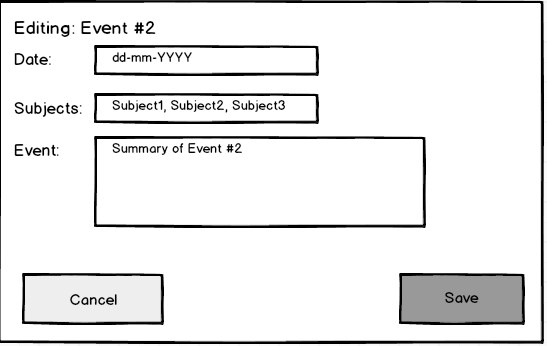
\includegraphics[scale=0.6]{editDialog.png}
\centering
\end{figure}
\begin{figure}[h]
\caption{Document Viewer of System}
\label{fig:viewDoc}
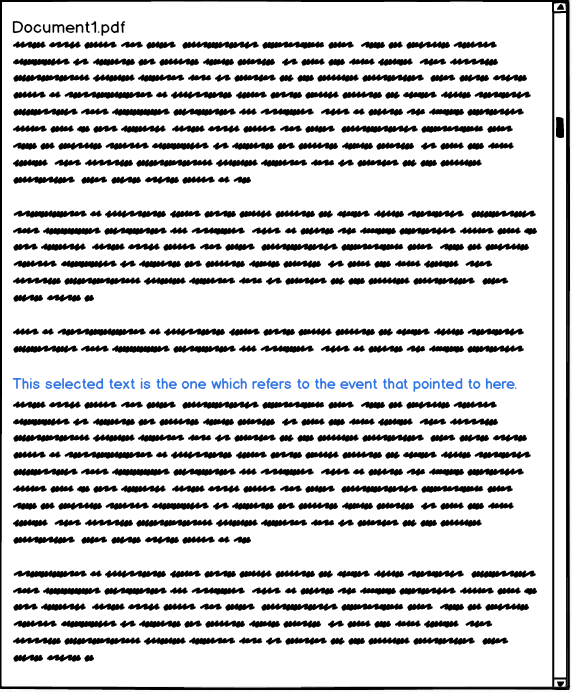
\includegraphics[scale=0.75]{viewDoc.png}
\centering
\end{figure}
\par In the Document Viewer (see Figure \ref{fig:viewDoc}), note that the relevant sentence that produced the event, which the user interacted with to view this, is highlighted. This allows the user to see in context the event, as they can read the text surrounding it, giving them a better understanding of what occurred. This also allows the user to swap between the system and the documents. In addition it allows the user to view how each event has been produced and judge for themselves how effective the system is. The user can also jump through the document using the timeline by selecting the view funtion from an event. Therefore, the user is no longer required to read the entire document or scroll through it if they are only interested in certain areas of it. This is extremely benefitial for large documents which are cumbersome to read, as the user can focus on specific areas of the document (i.e. the text surrounding the sentence that produced the event) instead of having to re-read the chapter, or even the whole document. Note the tool should not replace the reading of highly sensative and critical law documents (or any other kind of documents), as the user may require the full context of the document, but it can serve as a time-effective tool to skip through the document event-by-event, focusing on certain aspects of the documents being revisited.
//wireframes, reason for this, why no color, why no other layout?, update to new system










